\section{The Algorithm}
We start with a discussion of the algorithm of Jaiswal \etal\ \cite{jks} since our algorithm will be a modification of their algorithm.
Given a dataset $X$, let the optimal clusters be denoted by $X_1, ..., X_k$.
Suppose we have $i$ centers $C_i = \{c_1, ..., c_i\}$ such that these centers are good centers for some $i$ optimal clusters. 
That is, there exists distinct indices $j_1, ..., j_i \in \{1, ..., k\}$ such that $\forall l \leq i, \Phi_{c_l}(X_{j_l}) \leq (1 + O(\varepsilon)) \cdot \Delta(X_{j_l})$, where $\Delta(X_{j_l})$ denotes the optimal $1$-means cost of the cluster $X_{j_l}$.
Suppose at this time, we sample a set $S$ of $N$ points independently with the sampling technique of \kmpp. 
A formal description of \kmpp\ is given in Figure \ref{fig:kmpp}
Since the sampling technique gives preference to points that are further away from the current centers, we are likely to sample points from clusters whose indices do not appear in the set $\{j_1, ..., j_i\}$.
Let us call such clusters ``uncovered" clusters.
So, there is a good chance that a significant number of sampled points will be from uncovered clusters.
The algorithm of Jaiswal \etal\ \cite{jks} just considers all possible subset of points of size $M < N$ and considers the centroid of these points as the $(i+1)^{\textrm{th}}$ center. 
The main idea being that at least one of these subsets will behave as a uniform sample of points from some uncovered cluster and known results~\cite{inaba} suggests that the centroid of such a sample will be a good center for this uncovered cluster.
However, this results in the exponential running time since each time sampling is done, there are more than $1$ subsets to consider. 
\footnote{Even if we consider only two possibilities in each step, the running time will be $2^k$ since we have the sample $k$ times.}

\noindent
Our algorithm follows the same idea as that of Jaiswal~\etal\ \cite{jks} given in the above paragraph. 
However, while choosing the $(i+1)^{\textrm{th}}$ center, we do not try more than one possibility.
Instead of considering all possible subsets of $S$, we cluster $S$ into $k$ clusters using the \kmpp\ algorithm and then pick the centroid of the largest cluster as the $(i+1)^{th}$ center. 
\footnote{Ties are broken arbitrarily.}
Figure~\ref{fig:seed} gives a formal description of our algorithm. 
Figure~\ref{fig:illustration} gives an illustration of one iteration of our algorithm.
This algorithm has inherent data level parallelism. 
The parallel version of our algorithm is given in Figure~\ref{fig:par-seed}.
The rationale behind this choice for the $(i+1)^{th}$ center is the following: 
Let $X_l$ denote the uncovered cluster that is farthest from the current set $C_i$ of centers. That is, $\Phi_{C_i}(X_l)$ is the largest amongst the uncovered clusters. 
Note that $S$ is likely to have more points from $X_l$ than any other optimal cluster.
Ideally, we would like to isolate the points from $X_l$ present in $S$ and then take the centroid of these points. 
In Jaiswal~\etal\ \cite{jks} this was done by taking all possible subsets to ensure that one of these subsets contain all points from $X_l$. 
What we essentially do here is to cluster the points in $S$, the hope being that all points in $X_l$ that are present in $S$ will form a cluster.
Since our algorithm picks the largest cluster it would be able to isolate the points of $X_l$ present in $S$.

\noindent
Note that our suggested algorithm is a heuristic and we do not give any provable guarantees for our algorithm.
So, the only way to validate the effectiveness of our algorithm is to do a detailed experimental analysis on real and synthetic datasets. 
This is what we discuss in the remaining paper. 


\begin{center}
\begin{Algorithm}[h]
\begin{boxedminipage}{5.5in}
{\tt $D^2$-Seeding($X, k, N$)}

\hspace{0.1in} (1) $C_0 \leftarrow \{\}$

\hspace{0.1in} (2) For $i$ = $1$ to $k$

\hspace{0.3in} (a) Sample a multiset $S$ of $N$ points from $X$ using $D^2$ sampling with respect to $C_{i-1}$. \footnote{When $i=1$, $D^2$-sampling is the same as uniform sampling.}

\hspace{0.3in} (b) Let $T_l$ denote the largest cluster obtained by running \kmpp 

\hspace{0.3in}  \ \ \ \ \ \ algorithm on inputs $S$ and $k$.

\hspace{0.3in} (c) $c_i \leftarrow \Gamma(T_l)$ and $C_i \leftarrow C_{i-1} \cup \{c_i\}$. 
\footnote{$\Gamma(T)$ denote the centroid of the points in $T$ i.e., $\Gamma(T) = \frac{\sum_{t \in T} t}{|T|}$.}

\hspace{0.1in} (3) Output $C_k$
\end{boxedminipage}
\caption{Our seeding algorithm. $N$ is an input parameter that may be adjusted for performance/quality.}
\label{fig:seed}
\end{Algorithm}
\end{center}

\vspace{-0.4in}

\begin{center}
\begin{Algorithm}[h]
\begin{boxedminipage}{5.5in}
{\tt Par-$D^2$-Seeding($X, k, N$)}

\hspace{0.1in} (1) $C_0 \leftarrow \{\}$

\hspace{0.1in} (2) For all $1 \leq j \leq M$, let $P_j = \left\{X\left[{\frac{(j-1) \cdot |X|}{M}} \right], ..., X\left[{\frac{j \cdot |X|}{M}}\right]\right\}$. \footnote{$X[i]$ denotes the $i^{th}$ element of the dataset $X$}

\hspace{0.1in} (3) {\bf For} $i$ $\leftarrow$ $1$ to $k$:

%\hspace{0.3in} (a) {\bf Parfor} $j$ $\leftarrow$ $1$ to $M$

%\hspace{0.5in} (i) Sample a multiset $S_j$ of $N$ points from $P_j$ using $D^2$-sampling  with respect to $C_{i-1}$. 

\hspace{0.3in} (a) $S \leftarrow \{\}$ \ \ \ \ \ \ \ \ \ {\it // $S$ here denotes a multiset.}

\hspace{0.3in} (b) {\bf Parallel-for} $j \leftarrow 1$ to $M$:

\hspace{0.5in} (i) For all $1 \leq l \leq |X|/M$, $D_j[l] \leftarrow \Phi_{C_{i-1}}(\{P_j[l]\})$.

\hspace{0.5in} (ii) $D[j] \leftarrow \Phi_{C_{i-1}}(P_j)$.

\hspace{0.3in} (c) Let $\mathcal{D}$ denote the distribution over $\{1, ..., M\}$ defined by $D[1], ..., D[M]$.

\hspace{0.3in} (d) For all $j$, let $\mathcal{D}_j$ denote a distribution over $\left\{1, ..., \frac{|X|}{M} \right\}$ defined by $D_j[1], ..., D_j \left[\frac{|X|}{M}\right]$.


\hspace{0.3in} (e) {\bf Parallel-for} $j$ $\leftarrow$ $1$ to $N$:

\hspace{0.5in} (i) Sample $r$ from $\mathcal{D}$ and then $t$ from $\mathcal{D}_r$.

\hspace{0.5in} (ii) $S \leftarrow S \cup P_r[t]$.

\hspace{0.3in} (f) Let $T_l$ denote the largest cluster obtained by running \kmpp

\hspace{0.3in}  \ \ \ \ \ \ algorithm on inputs $S$ and $k$.

\hspace{0.3in} (g) $c_i \leftarrow \Gamma(T_l)$ and $C_i \leftarrow C_{i-1} \cup \{c_i\}$. 

\hspace{0.1in} (4) Output $C_k$
\end{boxedminipage}
\caption{Parallel version of our seeding algorithm. $N$ is an input parameter and $M$ is a global environment variable indicating the number of hardware-level threads available.}
\label{fig:par-seed}
\end{Algorithm}
\end{center}


\begin{figure}
\centering
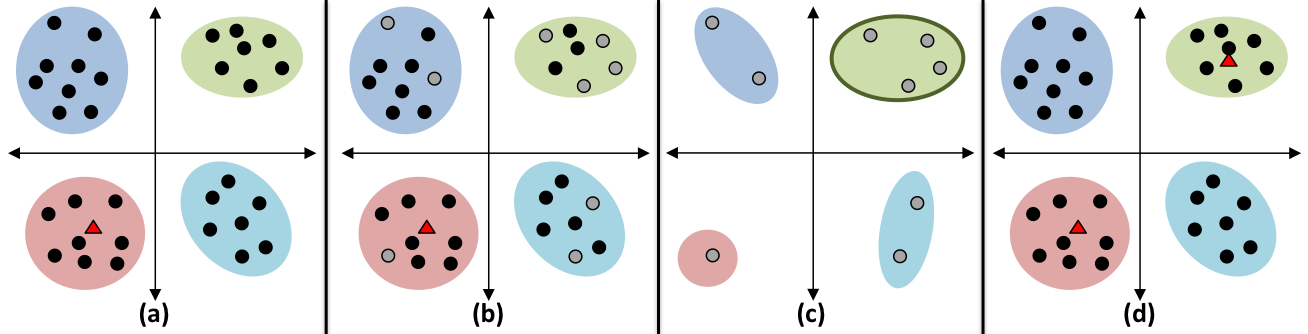
\includegraphics[scale=0.3]{illustration}
\caption{(a) First center (red triangle) has been chosen in iteration $1$ (b) Points (in gray) are sampled with $D^2$-sampling (c) The sampled points are clustered (d) Centroid of the largest cluster is chosen as the second center.}
\label{fig:illustration}
\end{figure}


